% Preamble
\documentclass[12pt]{article}

% Packages
\usepackage[left=3.0cm, right=1.5cm, top=2.0cm, bottom=2.0cm]{geometry}

\usepackage[utf8]{inputenc}
\usepackage[T2A]{fontenc}
\usepackage[russian]{babel}
\usepackage{amsmath, amsfonts, amssymb}
\usepackage{graphicx}
\usepackage{wrapfig}
\usepackage{fancyhdr}
\usepackage[shortlabels]{enumitem}
\usepackage{svg}
\usepackage{amstex}
\usepackage{colortbl}
\usepackage{bm}

\renewcommand{\vec}{\textbf}
\newcommand{\cross}{\times}

\pagestyle{fancy}
\fancyhead[L]{Работа №4.4.3}
\fancyhead[R]{Белинский Т.Д.\quad Б05-206}

% Document
\begin{document}
    \section*{4.4.3. ИЗУЧЕНИЕ ПРИЗМЫ\\С ПОМОЩЮ ГОНИОМЕТРА}
    \ \par
    \textbf{Цель работы:} знакомство с работой и настройкой гониометра Г5,
    определение зависимости показателя преломления стекла призмы от длины волны,
    определение марки стекла и спектральных характеристик призмы.

    \textbf{Оборудование:} гониометр, ртутная лампа, призма, стеклянная плоскопараллельная пластинка,
    призменный уголковый отражатель.

    \subsection*{Теоретическая часть}
    \ \par

    \begin{wrapfigure}[15]{r}{0.5\linewidth}
        \centering
        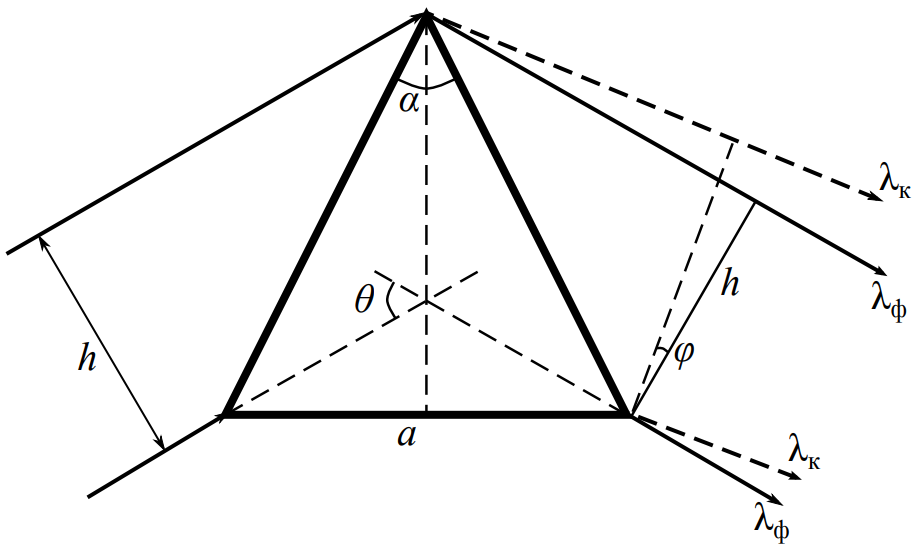
\includegraphics[width=0.8\linewidth]{pic/theory}
        \caption{Ход лучей в призме для угла наименьшего отклонения}
        \label{fig:fig1}
    \end{wrapfigure}

    Показатель преломления материала призмы $n(\lambda)$ удобно определять
    по углу наименьшего отклонения $\delta(\lambda)$ (рис.\ \ref{fig:fig1}).
    Минимальное отклонение луча, преломлённого призмой, от направления луча, падающего
    на призму, получается при симметричном ходе луча (в призме луч идёт
    параллельно основанию).

    Угол минимального отклонения $\delta$, преломляющий угол $\alpha$ (угол при вершине призмы) и показатель преломления
    связаны соотношением
    \begin{equation}
        \label{eq:eq1}
        n(\lambda) = \frac{\sin \frac{\alpha + \delta(\lambda)}{2}}{\sin \frac{\alpha}{2}}.
    \end{equation}


    \subsection*{Экспериментальная установка}
    \ \par
    \textbf{Устройство гониометра Г5.} Внешний вид гониометра представлен на рис.\ \ref{fig:fig2}.
    Коллиматор 3, столик 7 и алидада 17 со зрительной трубой 12 крепится на массивном основании 23.
    На столике 7 размещаются исследуемые объекты.
    Коллиматор закреплён неподвижно, а столик и алидада с трубой могут вращаться вокруг вертикальной оси.

    \begin{figure}[h]
        \centering
        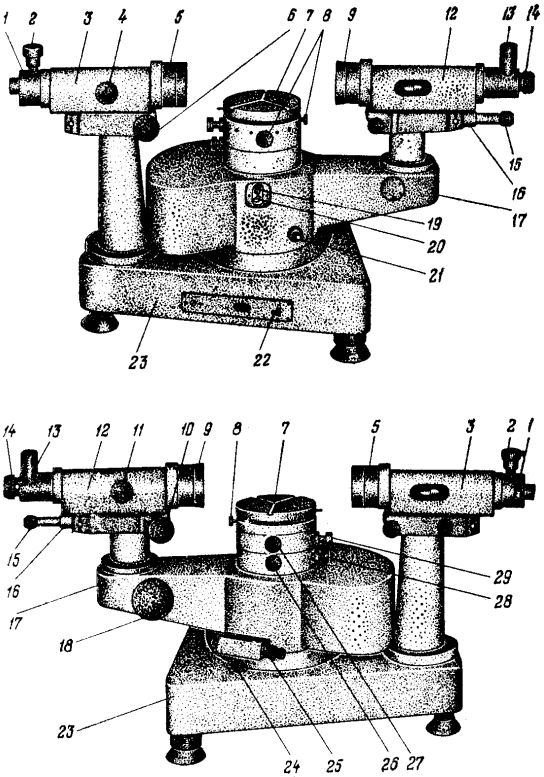
\includegraphics[width=0.6\linewidth]{pic/setup}
        \caption{Внешний вид гониометра Г5}
        \label{fig:fig2}
    \end{figure}

    Ширину коллиматорной щели можно менять от 0 до 2-х мм при помощи
    микрометрического винта 2, высоту — от 0 до 20 мм — при помощи диафрагмы с треугольным вырезом («ласточкин хвост»), надетой на щель. Винт 4 служит для настройки коллиматора на параллельный пучок. Зрительная труба
    12 состоит из объектива 9 и окуляра 14 с автоколлимационным устройством
    13. объективы коллиматора и зрительной трубы одинаковы.
    Фокусировка трубы производится винтом 11.
    Наклон коллиматора и зрительной трубы к горизонтально оси изменяется винтами 6 и 10 соответственно

    Важнейшим узлом гониометра является устройство,
    служащее для отсчёта угла поворота зрительной трубы вокруг вертикальной оси,
    проходящей через центр столика.
    На этой оси крепится прозрачное кольцо (лимб), расположенное в корпусе прибора.
    На поверхности лимба нанесена шкала с делениями.
    Лимб разделён на $3 \times 360 = 1080$ делений. Цена деления $20'$,
    оцифровка делений произведена через $1^{\circ}$.
    Шкалу лимба можно наблюдать через окуляр отсчётного устройства 16 при включённой подсветке (тумблер 22).
    Резкость изображения шкалы регулируется вращением оправы окуляра 15.

    Оптическая система отсчётного устройства собрана так, что через окуляр
    можно наблюдать изображения штрихов двух диаметрально противоположных участков лимба,
    причём одно изображение прямое, а другое обратное.
    Кроме того, оптическая система позволяет перемещать эти изображения друг относительно друга,
    оставляя в покое как лимб, так и алидаду со зрительной трубой.
    Это перемещение штрихов измеряется при помощи оптического микрометра.
    Шкала микрометра рассчитана таким образом, что при перемещении её на 600 делений
    верхнее изображение штрихов лимба смещается относительно нижнего на $10'$.
    Следовательно, цена деления шкалы микрометра $1''$.

    \subsection*{Результаты и обработка}
    \begin{enumerate}
        \item Измерение преломляющего угла:
        \begin{enumerate}
            \item устанавливаем зрительную трубу перпендикулярно одной из
            преломляющих граней призмы;
            \item записываем угловую координату;
            \item повторяем пункты (a) и (b) для второй преломляющей грани,
            результаты измерений приведены в таблице\ \ref{tab:tab1}.
        \end{enumerate}
        По итогам измерений преломляющий угол $\alpha = 180^{\circ} - |n_1 - n_2|$:
        \[\alpha = 63^{\circ}10'6'' \pm 10''\]
        \item Исследование спектра ртутной лампы:
        \begin{enumerate}
            \item поворачиваем столик с призмой и зрительную трубу так,
            чтобы в последней можно было увидеть линии спектра;
            \item затем вращая столик ищем положение,
            при котором отклонение линии спектра, видимой в зрительной трубе,
            от оси окуляра оказывается наименьшим;
            \item измеряем координату линии в данном положении;
            \item повторяем пункты (a) - (c) для 8 линий спектра,
            полученные данные приведены в таблице\ \ref{tab:tab2}.
        \end{enumerate}
        Для того чтобы получить значения углов наименьшего отклонения ($\delta$),
        необходимо вычесть координаты спектральных линий из координаты начала отсчета
        (направления на окуляр):
        \[\phi_0 = 180^{\circ}44'40'' \pm 5''.\]
        Показатели преломления оцениваются по формуле\ \eqref{eq:eq1}.
        \item По результатам эксперимента был построен график $n(\lambda)$ (рис.\ \ref{fig:fig3}).
        Как видно первые 6 точек хорошо аппроксимируются прямой с угловым коэффициентом
        \[\frac{dn}{d\lambda} = (2.1 \pm 0.1) \cdot 10^{3}\ \text{см}^{-1}\]
        \item По измерениям координат желтой пары рассчитаем угловую дисперсию:
        \[\frac{\Delta \phi}{\Delta \lambda} = (0.057 \pm 0.002)\ \frac{^{\circ}}{\text{нм}}\]
        \item Дисперсия решетки, имеющей 100 штр/мм (т.е. $b = 0.01$ мм), в первом порядке ($m = 1$)
        вычисляется по формуле:
        \[\frac{\Delta \phi}{\Delta \lambda} = \frac{m}{b \cos\theta_m} = 0.1 \cdot 10^{-3}\ \frac{^{\circ}}{\text{нм}},\]
        где $\theta_m \approx \frac{\lambda}{b}$.
        \item Оценим максимальную разрешающую способность призмы:
        \[R = a \left|\frac{dn}{d\lambda}\right| \approx 15330,\]
        где $a = 7.3$ см -- длина основания призмы.
    \end{enumerate}

    \begin{figure}
        \centering
        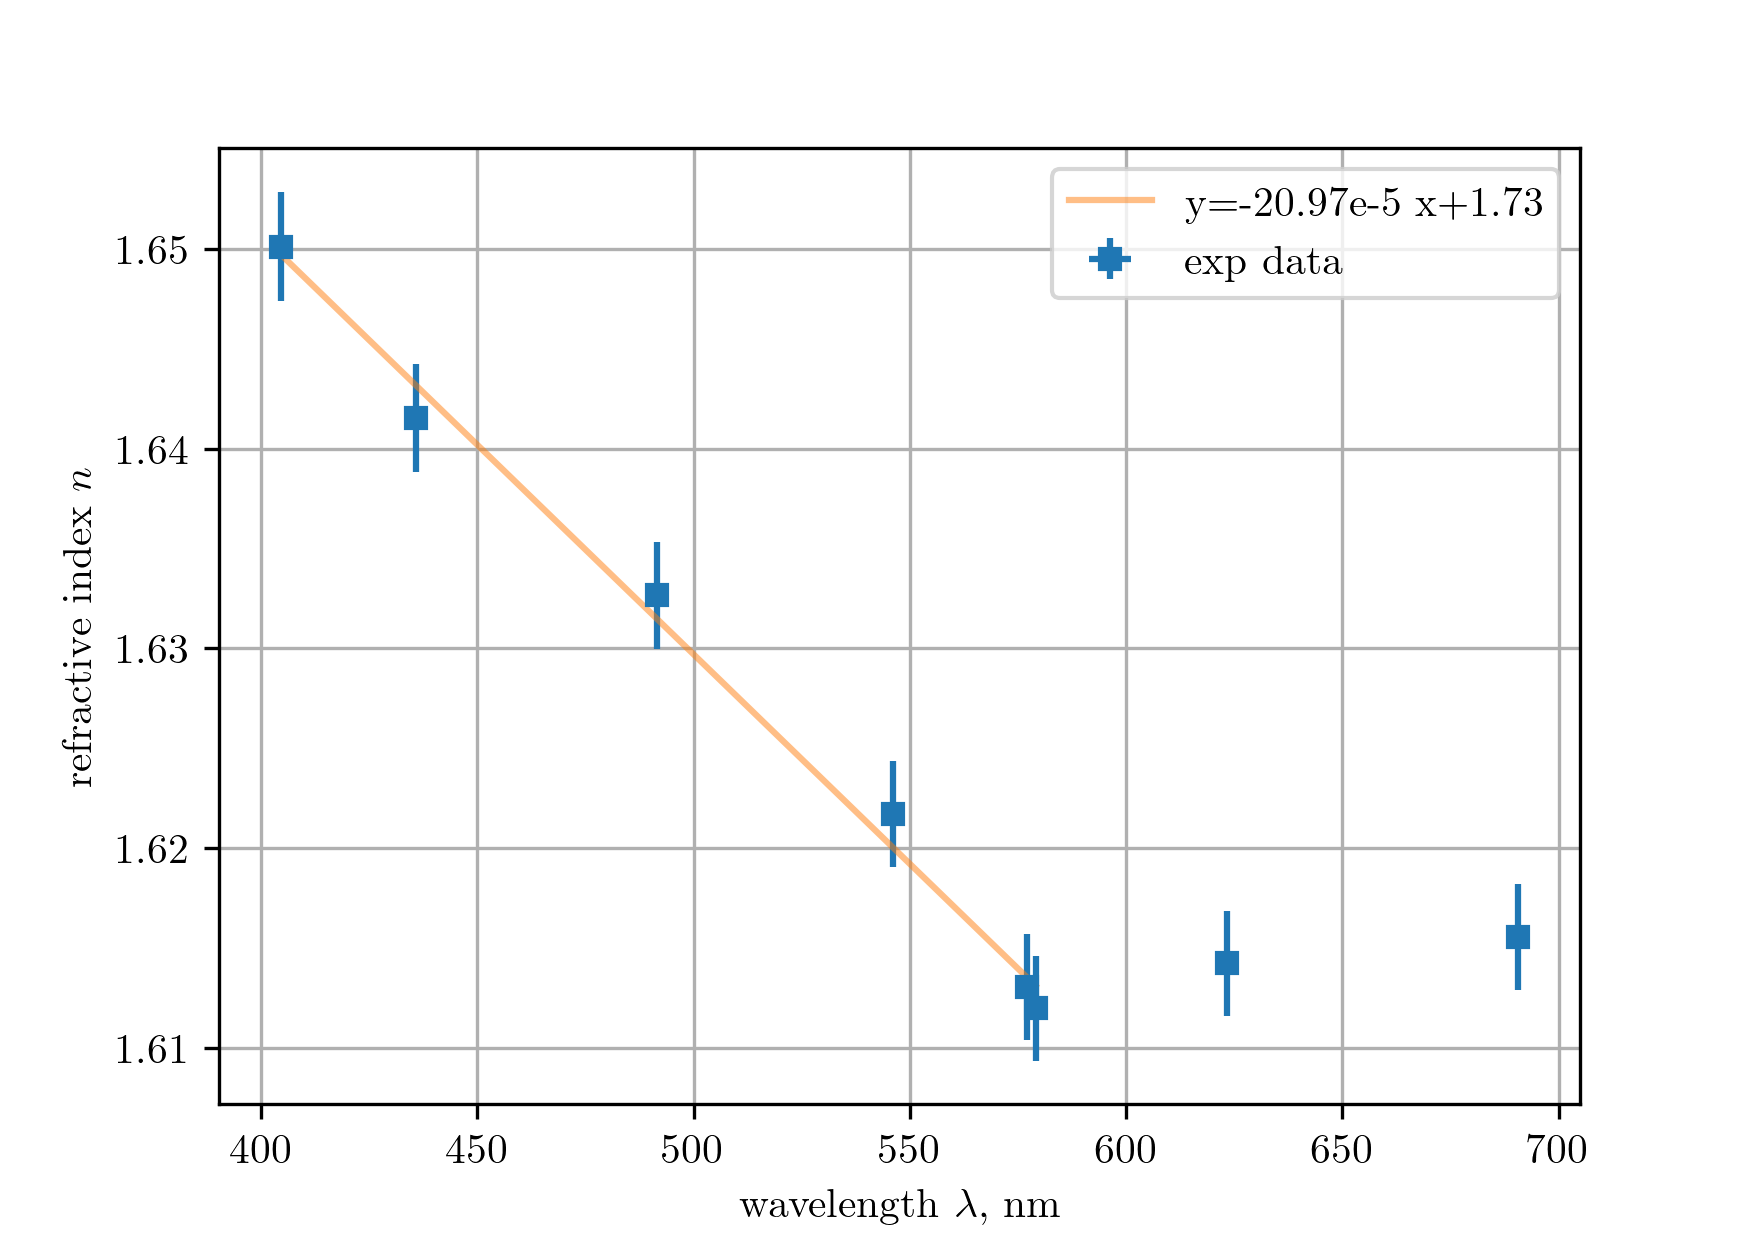
\includegraphics[width=0.8\linewidth]{pic/n(lmbd)}
        \caption{Зависимость показателя преломления от длины волны}
        \label{fig:fig3}
    \end{figure}


    \begin{table}
        \centering
        \caption{Координаты нормалей преломляющих граней}
        \label{tab:tab1}
        \begin{tabular}{|l|c|c|}
            \hline
            № & $n_1$                & $n_2$                \\\hline
            1 & $172^{\circ}34'47''$ & $289^{\circ}24'41''$ \\
            \hline
        \end{tabular}
    \end{table}

    \begin{table}
        \centering
        \caption{Координаты спектральных линий}
        \label{tab:tab2}
        \begin{tabular}{|l|c|c|c|c|c|}
            \hline
            № & $\lambda$, нм & $\phi$ (прямые измерения) & $\delta,\ ^{\circ}$ &
            n & \sigma_n \\\hline
            0 & 579.1 & $128^{\circ}43'25''$ & 52.021 & 1.612 & 0.003 \\
            1 & 577.0 & $128^{\circ}36'14''$ & 52.141 & 1.613 & 0.003 \\
            2 & 546.1 & $127^{\circ}37'35''$ & 53.118 & 1.622 & 0.003 \\
            3 & 491.6 & $126^{\circ}22'13''$ & 54.374 & 1.633 & 0.003 \\
            4 & 435.8 & $125^{\circ}20'5''$  & 55.410 & 1.642 & 0.003 \\
            5 & 404.7 & $124^{\circ}19'10''$ & 56.425 & 1.650 & 0.003 \\
            6 & 690.7 & $128^{\circ}19'23''$ & 52.421 & 1.616 & 0.003 \\
            7 & 623.4 & $128^{\circ}28'19''$ & 52.272 & 1.614 & 0.003 \\
            \hline
        \end{tabular}
    \end{table}

    \subsection*{Выводы}
    \begin{itemize}
        \item В данной работе измерен преломляющий угол лабораторной призмы:
        \[\alpha = 63^{\circ}10'6'' \pm 10'',\]
        а также оценена средняя дисперсия показателя преломления
        \[\frac{dn}{d\lambda} = (2.1 \pm 0.1) \cdot 10^{3}\ \text{см}^{-1}.\]
        Сверяясь со справочными значениями, стекло марки ТФ1
        обладает дисперсией $1.9 \cdot 10^3\ \text{см}^{-1}.$
        \item Угловая дисперсия призмы по результатам опыта составила:
        \[\frac{\Delta \phi}{\Delta \lambda} = (0.057 \pm 0.002)\ \frac{^{\circ}}{\text{нм}}\]
        \item Экспериментально измеренная разрешающая способность:
        \[R = \frac{\lambda}{\delta \lambda} \approx 300,\]
        что соответсвует реально работуещему размеру призмы:
        \[a = R \left|\frac{dn}{d\lambda}\right| ^{-1} \approx 0.2\ \text{мм}\]
    \end{itemize}

    \begin{minipage}[b]{\linewidth}
        \centering
        \begin{minipage}[b]{0.3\linewidth}
            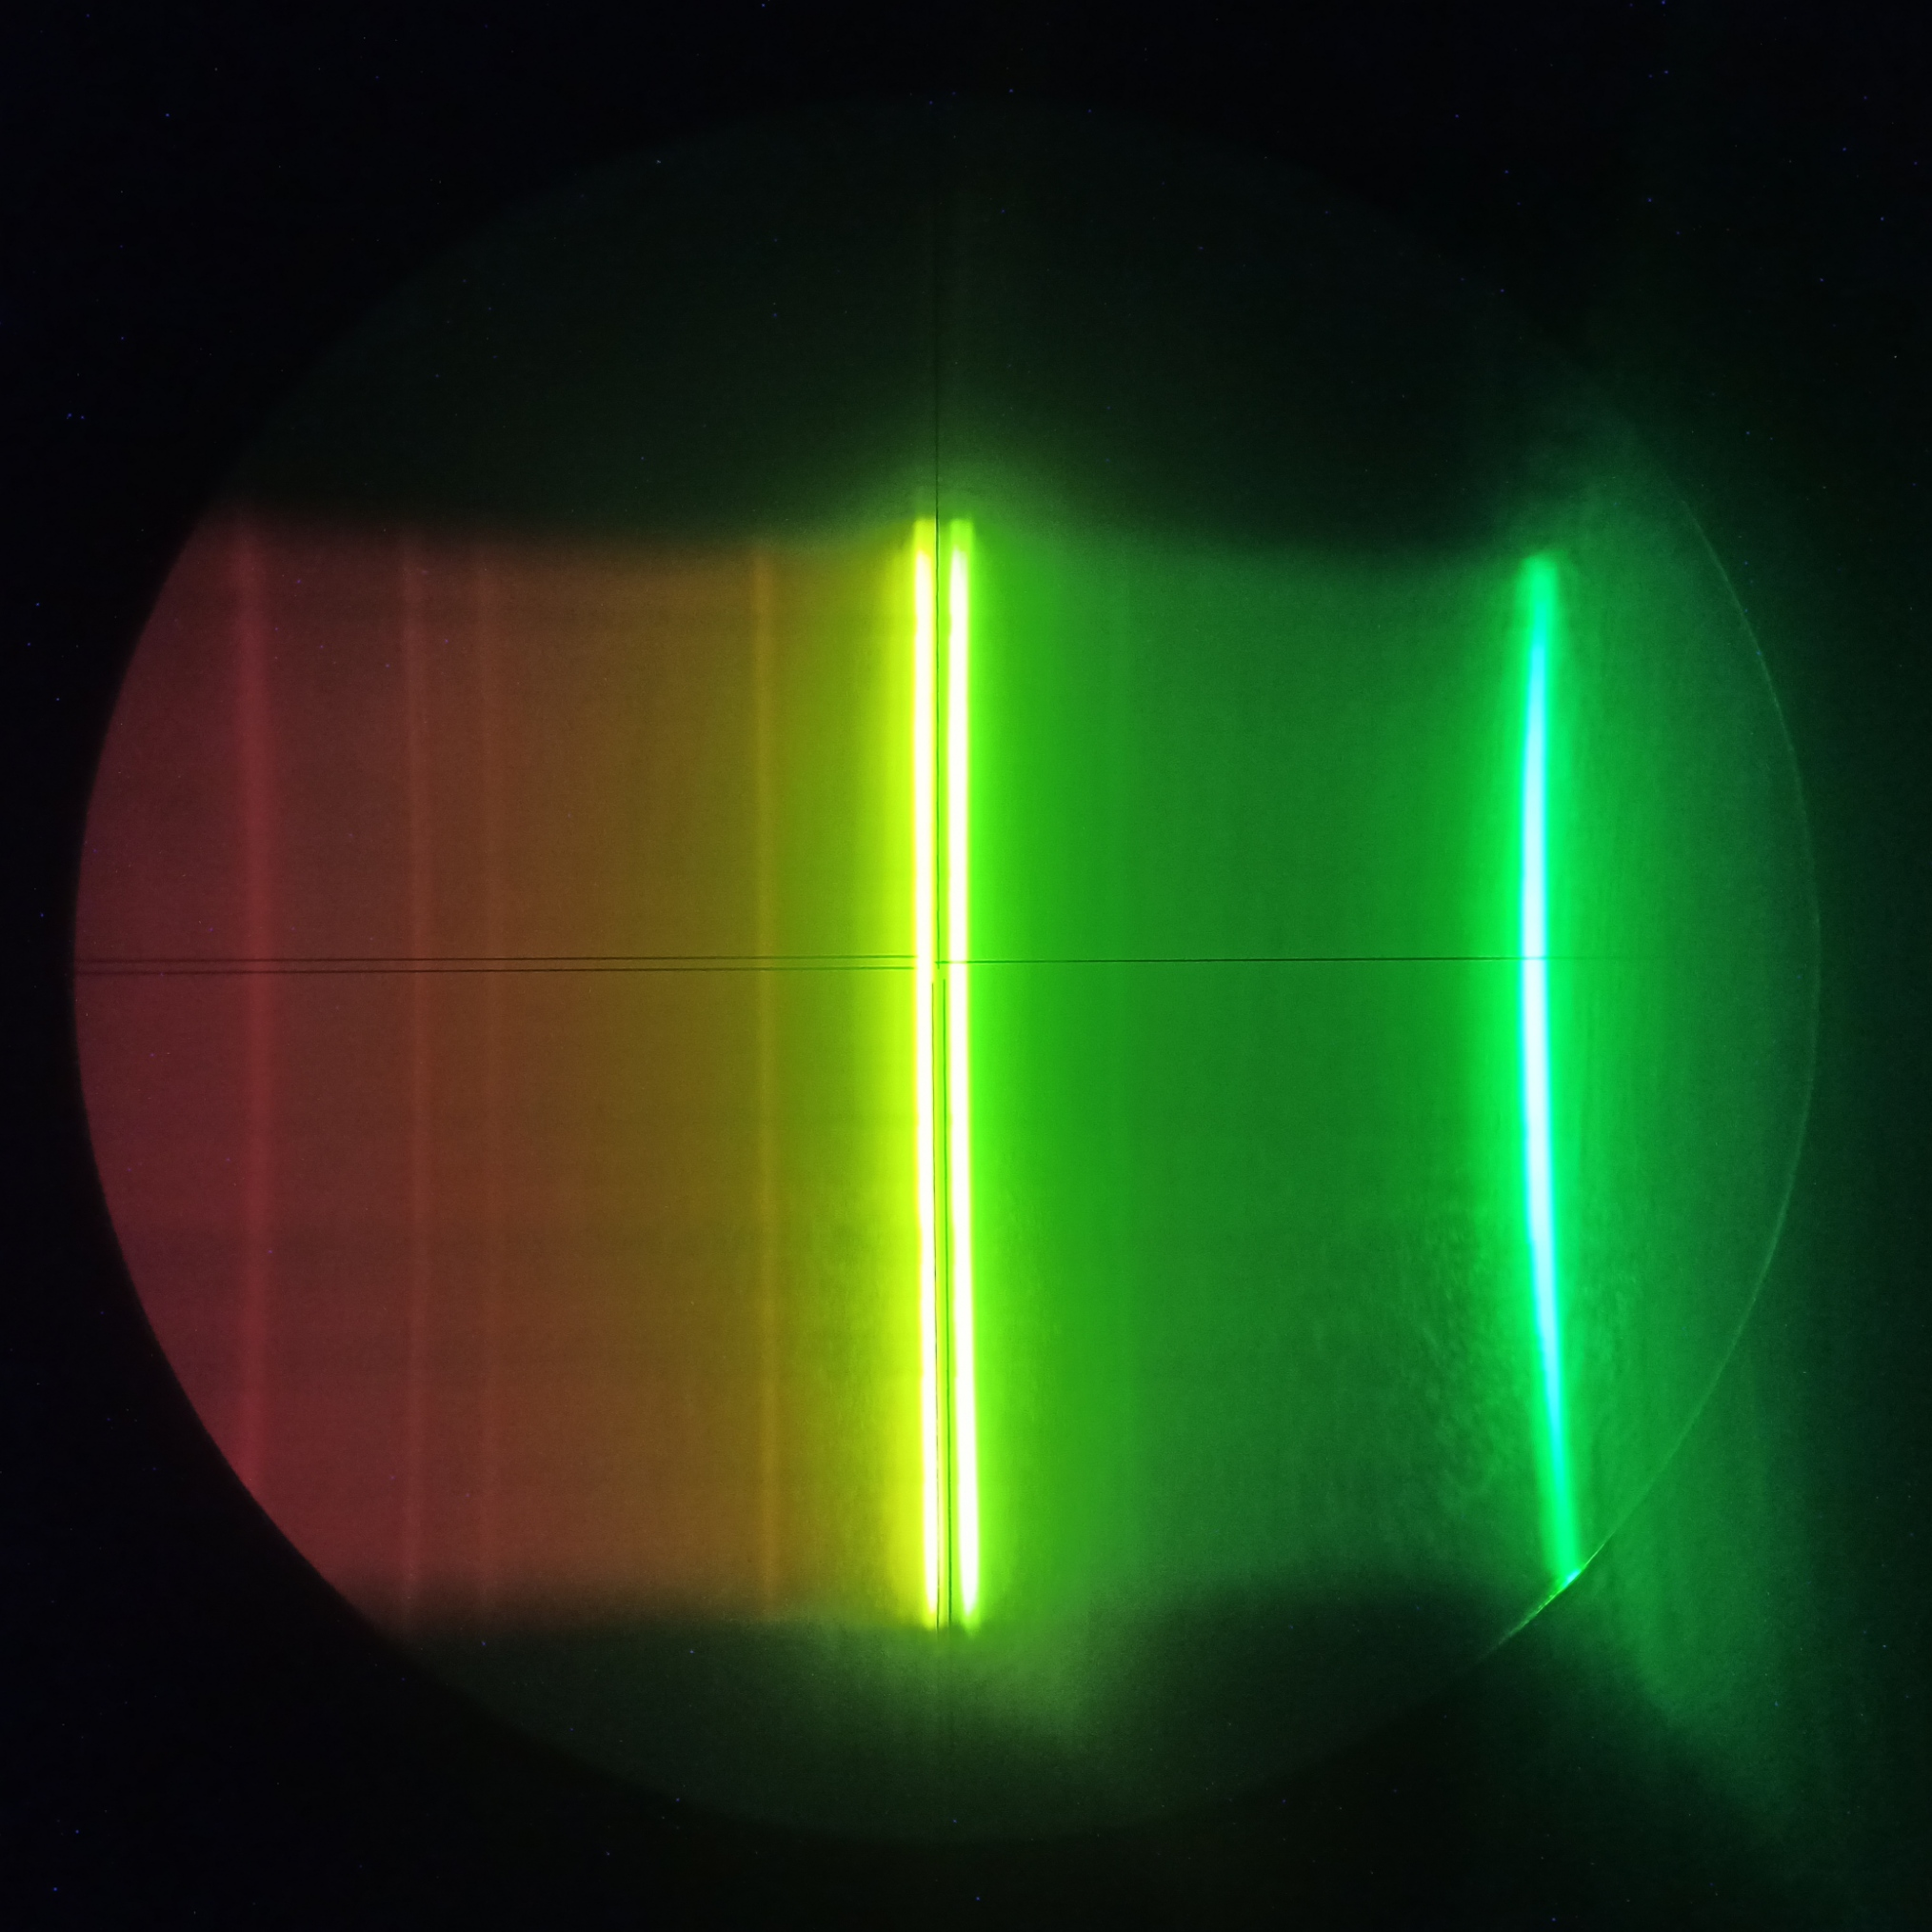
\includegraphics[width=\linewidth]{pic/1}
        \end{minipage}
        \begin{minipage}[b]{0.3\linewidth}
            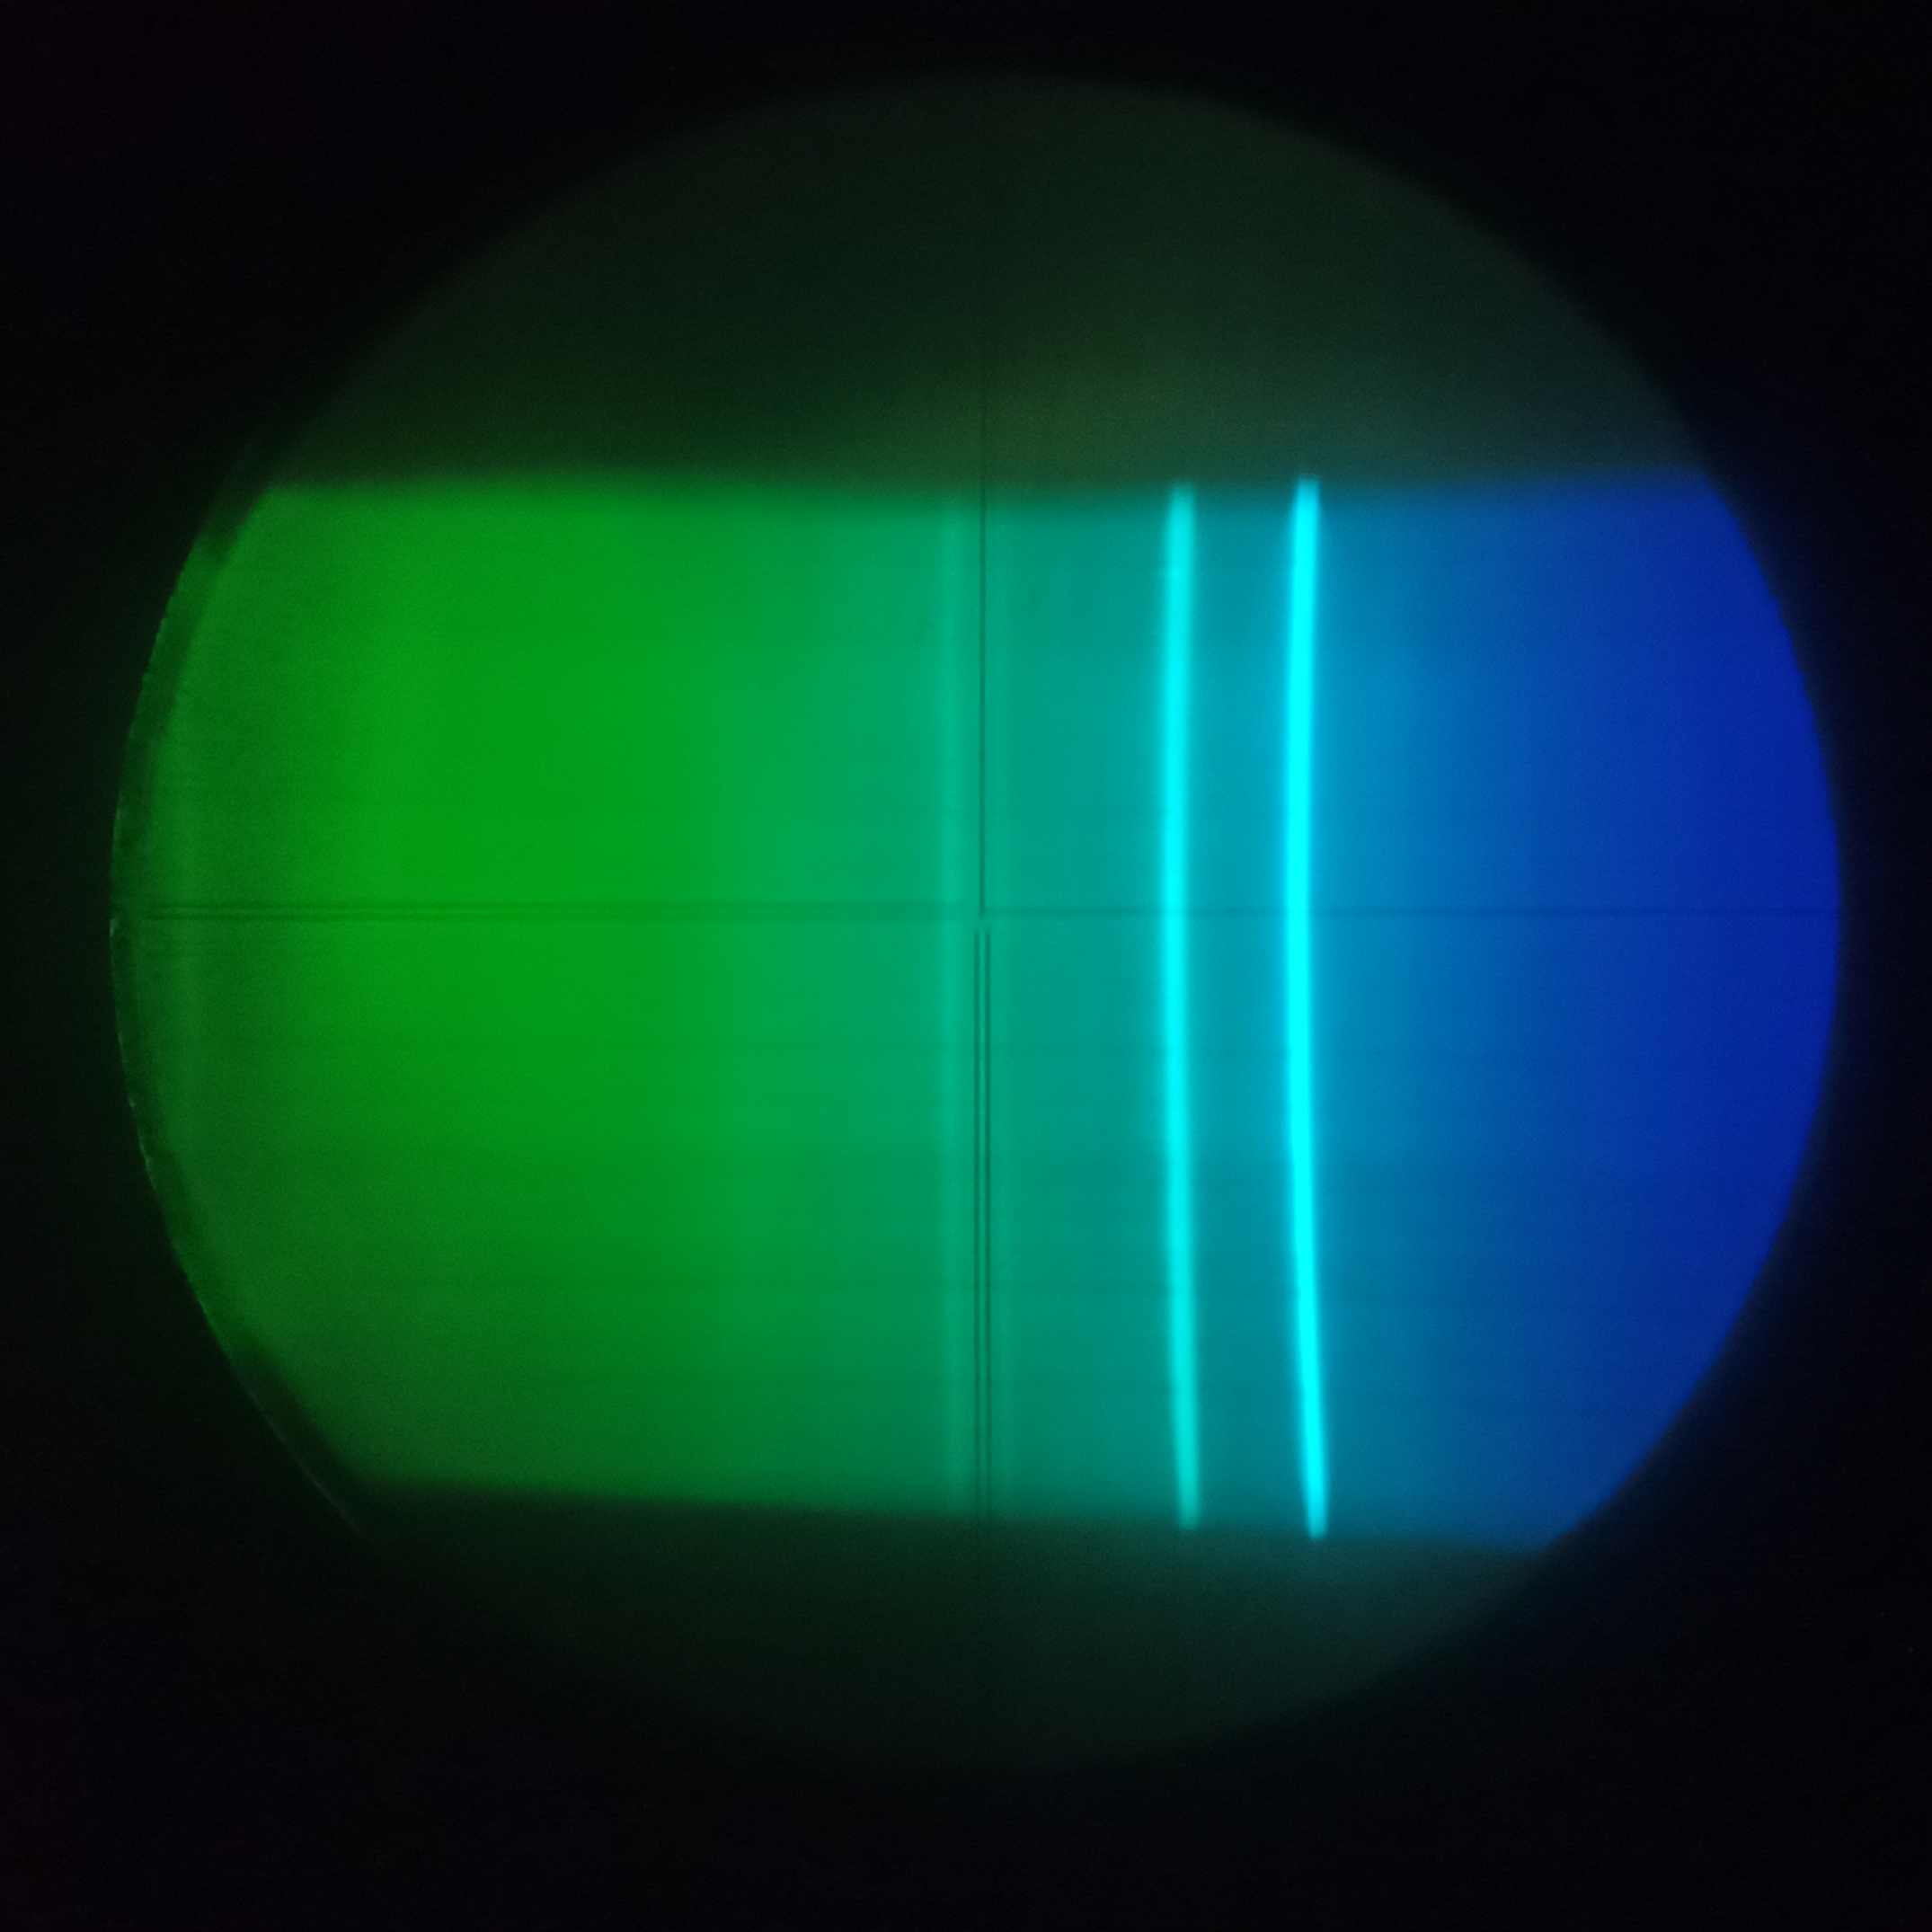
\includegraphics[width=\linewidth]{pic/2}
        \end{minipage}

        \caption{Рис. 4: Фотографии спектра ртутной лампы}
    \end{minipage}
\end{document}